\documentclass[aspectratio=43,11pt]{beamer}

% ================================================================
% Presentación de TP3 — Billar-Metegol (72.25, ITBA).
% Estilo heredado de TP2/presentacion/template_presentacion_tp2.tex.
% Compilar con: latexmk -pdf presentacion_imagen.tex
% ================================================================

% ----------------------------------------------------------------
% REVISAR A MANO antes de aceptar (corrección real de TP2: un label
% de eje sobrecargado "suena a eje nombrado por la IA"). Convención
% acordada para TODAS las figuras de esta presentación:
%   eje temporal .......... t [s]
%   cantidad de partículas  N
%   tiempo al 90% ......... ⟨t₉₀⟩ [s]
%   fracción usada ........ F_u
%   desplazamiento cuad. .. DCM [m²]
%   posición del obstáculo  x_k [m]
% Nada de paréntesis explicativos ni unidades del modelo entre
% corchetes. Si un label no entra en dos o tres símbolos, está mal.
%
% TAMAÑO DE FUENTE (corrección real de TP2: "los tamaños de fuente de
% las figuras son ilegibles"): la letra dentro de cada figura tiene que
% ser comparable a la del resto de la diapositiva. Si no se lee
% proyectada, está mal, sea cual sea el tamaño en puntos.
%
% NUNCA un título adentro del área graficada: eso va en el
% \frametitle. Los parámetros fijos van en el \parambox del costado,
% nunca repetidos en cada entrada de leyenda.
% ----------------------------------------------------------------

\usepackage[T1]{fontenc}
% "provide=*" permite compilar también en instalaciones mínimas de TeX Live.
\usepackage[provide=*,spanish]{babel}
\usepackage{lmodern}
\usepackage{amsmath,amssymb,bm}
\usepackage{graphicx}
\usepackage{tikz}
\usetikzlibrary{arrows.meta,calc,positioning}
% Para controlar leftmargin/itemsep/topsep del itemize angosto de \parambox
% (0.27\textwidth) -- el itemize default de beamer queda con demasiado
% margen y espaciado para una caja tan chica.
\usepackage{enumitem}

% ---------- Colores ----------
\definecolor{TPBlue}{HTML}{3939B5}
\definecolor{TPBlueDark}{HTML}{29298A}
\definecolor{TPBlack}{HTML}{050505}
\definecolor{TPNavGray}{HTML}{858585}
\definecolor{TPLight}{HTML}{E9E9F2}
\definecolor{TPPlaceholder}{HTML}{F4F4F7}
\definecolor{TPFresca}{HTML}{2E5FD0}
\definecolor{TPUsada}{HTML}{C0392B}
\definecolor{TPObstaculo}{HTML}{BFBFBF}

\setbeamercolor{normal text}{fg=black,bg=white}
\setbeamercolor{structure}{fg=TPBlue}
\setbeamercolor{frametitle}{fg=white,bg=TPBlue}
\setbeamercolor{itemize item}{fg=TPBlue}
\setbeamercolor{itemize subitem}{fg=TPBlue}
\setbeamercolor{title box}{fg=white,bg=TPBlue}
\setbeamercolor{databox title}{fg=white,bg=TPBlueDark}
\setbeamercolor{databox body}{fg=black,bg=TPLight}
\setbeamercolor{algorithm box}{fg=black,bg=white}
\setbeamercolor{headline navigation}{fg=TPNavGray,bg=TPBlack}
\setbeamertemplate{items}[circle]
\setbeamertemplate{navigation symbols}{}

\setbeamerfont{frametitle}{size=\Large,series=\mdseries}
\setbeamerfont{normal text}{size=\normalsize}
\setbeamerfont{itemize/enumerate body}{size=\normalsize}
\setbeamerfont{itemize/enumerate subbody}{size=\small}

% ---------- Metadatos ----------
\title{Trabajo Práctico Nro.3: Simulación Dirigida por Eventos}
\subtitle{72.25 - Simulación de Sistemas}
\author{%
  Federico Ignacio Ruckauf\texorpdfstring{\textsuperscript{1}}{1}
  \and Federico Spivak Fontaiña\texorpdfstring{\textsuperscript{2}}{2}
  \and Lorenzo Chiossone\texorpdfstring{\textsuperscript{3}}{3}%
}
\institute{Instituto Tecnológico de Buenos Aires}
\date{2026 2C --- Grupo N.º 02}

% URLs de las animaciones (diapositivas 16 y 27).
% COMPLETAR cuando los videos estén subidos a YouTube.
\newcommand{\animacionVaciaURL}{https://youtu.be/COMPLETAR}
\newcommand{\animacionElegidaURL}{https://youtu.be/COMPLETAR}

% Si existe logo_itba.png o logo_itba.pdf junto al .tex, se inserta.
\newcommand{\institutionlogo}{%
  \IfFileExists{logo_itba.pdf}{
\includegraphics[height=0.75cm]{logo_itba.pdf}}{%
    \IfFileExists{logo_itba.png}{
\includegraphics[height=0.75cm]{logo_itba.png}}{%
      \fbox{\scriptsize LOGO DE LA INSTITUCIÓN}%
    }%
  }%
}

% ---------- Barra superior por sección ----------
% Rangos de diapositivas:
% Introducción 2--5 (incluye Modelo, fusionado -- ver TP2) | Implementación 6--9
% Simulaciones 10--13 | Resultados 14--30 | Conclusiones 31--33
% Cada rango incluye su \sectiondivider como primera diapositiva del
% bloque. Si se agregan o quitan diapositivas hay que renumerar estos
% rangos a mano.
\newcount\TPNavDot

\newcommand{\navdots}[2]{%
  \begingroup
    \TPNavDot=#1\relax
    \loop
      \ifnum\insertframenumber=\TPNavDot
        \raisebox{0.45mm}{{\color{white}\fontsize{6}{6}\selectfont$\bullet$}}%
      \else
        \raisebox{0.45mm}{{\color{TPNavGray}\fontsize{7}{7}\selectfont$\circ$}}%
      \fi
      \ifnum\TPNavDot<#2\relax
        \kern0.60mm
        \advance\TPNavDot by 1\relax
    \repeat
  \endgroup
}

\newcommand{\navblock}[4]{%
  % #1 ancho, #2 nombre, #3 inicio, #4 fin
  \makebox[#1\paperwidth][c]{%
    \parbox[c][0.62cm][c]{#1\paperwidth}{%
      \centering
      \ifnum\insertframenumber>1
        \ifnum\insertframenumber<#3
          {\color{TPNavGray}\scriptsize\strut #2}%
        \else
          \ifnum\insertframenumber>#4
            {\color{TPNavGray}\scriptsize\strut #2}%
          \else
            {\color{white}\scriptsize\strut #2}%
          \fi
        \fi
      \else
        {\color{TPNavGray}\scriptsize\strut #2}%
      \fi
      \par\vspace{-0.55mm}
      \navdots{#3}{#4}%
    }%
  }%
}

% Fila de navegación por secciones -- factorizada para no duplicarla
% entre las dos ramas de \TPheadline (con y sin franja de relleno).
\newcommand{\TPnavrow}{%
  \makebox[\paperwidth][l]{%
    \navblock{0.21}{Introducción}{2}{5}%
    \navblock{0.19}{Implementación}{6}{9}%
    \navblock{0.17}{Simulaciones}{10}{13}%
    \navblock{0.26}{Resultados}{14}{30}%
    \navblock{0.17}{Conclusiones}{31}{33}%
  }%
}

% La franja azul de relleno (para diapositivas sin título, ej.
% \sectiondivider) NUNCA debe cambiar la altura TOTAL del headline: si se
% suma como una caja extra arriba de la altura de la barra de navegación
% normal, el headline queda 0.05cm (~1.42pt) más alto que en las
% diapositivas con título, y LaTeX no tiene margen para absorberlo en los
% frames centrados verticalmente ([c], o con \vfill como portada/cierre)
% -- produce "Overfull \vbox (1.42271pt too high)" y una línea residual
% visible en el borde superior. Por eso la franja le resta exactamente lo
% mismo que ocupa al "dp" de la barra de navegación (0.28cm -> 0.23cm):
% el total (barra + franja) da siempre 0.78cm, igual que una diapositiva
% con título.
\setbeamertemplate{headline}{%
  \leavevmode
  \ifdefempty{\insertframetitle}{%
    \begin{beamercolorbox}[wd=\paperwidth,ht=0.50cm,dp=0.23cm]{headline navigation}%
      \TPnavrow
    \end{beamercolorbox}%
    \par\nointerlineskip
    \begin{beamercolorbox}[wd=\paperwidth,ht=0.05cm,dp=0cm]{frametitle}\end{beamercolorbox}%
  }{%
    \begin{beamercolorbox}[wd=\paperwidth,ht=0.50cm,dp=0.28cm]{headline navigation}%
      \TPnavrow
    \end{beamercolorbox}%
  }%
}

\setbeamertemplate{frametitle}{%
  \nointerlineskip
  \begin{beamercolorbox}[wd=\paperwidth,ht=0.74cm,dp=0.12cm,leftskip=0.35cm]{frametitle}
    \usebeamerfont{frametitle}\insertframetitle
  \end{beamercolorbox}
}

\setbeamersize{text margin left=0.55cm,text margin right=0.55cm}

% Pie mínimo con número de diapositiva.
\setbeamertemplate{footline}{%
  \leavevmode
  \hbox{\begin{beamercolorbox}[wd=\paperwidth,ht=0.20cm,dp=0.10cm,rightskip=0.18cm]{normal text}
    \hfill{\color{TPNavGray}\tiny\insertframenumber/\inserttotalframenumber}
  \end{beamercolorbox}}
}

% ---------- Componentes reutilizables (heredados de TP2) ----------
\newcommand{\sectiondivider}[1]{%
  \begin{frame}[c]{}
    \makebox[\linewidth][c]{%
      \begin{beamercolorbox}[wd=0.56\paperwidth,ht=0.55cm,dp=0.15cm,center]{frametitle}
        \large #1
      \end{beamercolorbox}%
    }
  \end{frame}
}

\newcommand{\placeholder}[2][4.4cm]{%
  \begingroup
    \setlength{\fboxsep}{0pt}%
    \setlength{\fboxrule}{0.45pt}%
    \fcolorbox{TPNavGray}{TPPlaceholder}{%
      \parbox[c][\dimexpr#1-2\fboxrule\relax][c]{%
        \dimexpr\linewidth-2\fboxrule\relax}{%
        \centering\color{TPNavGray}\small #2}%
    }%
  \endgroup
}

\newcommand{\maybeimage}[3]{%
  \IfFileExists{#1}{\includegraphics[width=\linewidth,height=#2,keepaspectratio]{#1}}{%
    \placeholder[#2]{#3\\[2mm]\nolinkurl{#1}}%
  }%
}

% Ambas versiones muestran debajo un enlace visible a YouTube.
% En la versión YouTube, además, la propia imagen funciona como enlace.
\newcommand{\videooimagen}[4]{%
  \begin{minipage}{\linewidth}
    \centering
    \ifdefined\versionyoutube
      \href{#3}{\maybeimage{#1}{#2}{#4}}%
    \else
      \maybeimage{#1}{#2}{#4}%
    \fi
    \par\vspace{1mm}
    \href{#3}{{\color{TPBlue}\scriptsize\nolinkurl{#3}}}%
  \end{minipage}%
}

% Caja de parámetros fijos, en la columna derecha (~28% del frame) --
% nunca repetidos dentro de la leyenda (corrección real de TP2). Lista de
% viñetas alineada a la izquierda (no centrada): el contenido se pasa como
% una secuencia de \item, ej. \parambox{\item A \item B \item C}.
\newcommand{\parambox}[1]{%
  \begin{beamercolorbox}[wd=\linewidth,sep=2mm]{databox body}
    \small
    \begin{itemize}[label=\textcolor{TPBlue}{$\bullet$},leftmargin=3.2mm,labelsep=1mm,itemsep=1mm,topsep=0pt,parsep=0pt]
      #1
    \end{itemize}
  \end{beamercolorbox}%
}

% Una animación por diapositiva, con la caja de parámetros al costado
% (columns, igual patrón que D3 "Sistema Real y Objetivo"). En TP2 era
% \dobleanimacion, con dos animaciones lado a lado; acá se compara una
% configuración por vez, así que el costado queda libre para \parambox.
% #1 imagen, #2 altura, #3 URL, #4 texto del placeholder, #5 parámetros fijos.
\newcommand{\animacionsimple}[5]{%
  \begin{columns}[T,onlytextwidth]
    \begin{column}{0.70\textwidth}
      \videooimagen{#1}{#2}{#3}{#4}%
    \end{column}
    \begin{column}{0.27\textwidth}
      \parambox{#5}%
    \end{column}
  \end{columns}%
}

% Diapositiva de resultados: figura a la izquierda (0.70) y, a la derecha,
% la caja de parámetros fijos y opcionalmente un mapa de ejemplo de la
% familia de configuraciones barrida, con su epígrafe.
% #1 figura, #2 altura, #3 texto del placeholder, #4 parámetros fijos,
% #5 mapa (vacío = sin mapa), #6 epígrafe del mapa.
\newcommand{\resultadofigura}[6]{%
  \begin{columns}[T,onlytextwidth]
    \begin{column}{0.70\textwidth}
      \centering
      \maybeimage{#1}{#2}{#3}%
    \end{column}
    \begin{column}{0.27\textwidth}
      \parambox{#4}%
      \ifstrempty{#5}{}{%
        \par\vspace{2mm}\centering
        \maybeimage{#5}{2.1cm}{Mapa de ejemplo}\par
        {\scriptsize\color{TPNavGray}#6\par}%
      }%
    \end{column}
  \end{columns}%
}

\newenvironment{databox}[1]{%
  \begin{beamercolorbox}[wd=\linewidth,sep=1mm,center]{databox title}%
    #1
  \end{beamercolorbox}%
  \par\nointerlineskip
  \begin{beamercolorbox}[wd=\linewidth,sep=2mm]{databox body}%
}{%
  \end{beamercolorbox}%
}

% ================================================================
% PRESENTACIÓN
% ================================================================
\begin{document}

% 1. PORTADA
\begin{frame}{}
  \vspace{0.35cm}
  \begingroup
    \makebox[\linewidth][c]{%
      \begin{beamercolorbox}[wd=0.91\linewidth,sep=3mm,center]{title box}
        \resizebox{0.92\linewidth}{!}{\strut\inserttitle}\par
        \vspace{1mm}
        {\large\insertsubtitle}
      \end{beamercolorbox}%
    }
    \par
  \endgroup
  \vspace{0.35cm}
  \begin{center}
    {\small\insertauthor\par}
    \vspace{0.18cm}
    {\scriptsize
      \textsuperscript{1}\href{mailto:fruckauf@itba.edu.ar}{fruckauf@itba.edu.ar}\\[0.5mm]
      \textsuperscript{2}\href{mailto:fespivak@itba.edu.ar}{fespivak@itba.edu.ar}\\[0.5mm]
      \textsuperscript{3}\href{mailto:lchiossone@itba.edu.ar}{lchiossone@itba.edu.ar}
      \par
    }
    \vspace{0.13cm}
    {\small\insertinstitute\par}
    \vspace{0.35cm}
    {\large\insertdate\par}
    \vfill
    \institutionlogo
  \end{center}
\end{frame}

% ---------------- INTRODUCCIÓN ----------------
% 2
\sectiondivider{Introducción}

% 3
\begin{frame}{Sistema Real y Objetivo}
  \begin{columns}[T,onlytextwidth]
    \begin{column}{0.53\textwidth}
      \small
      Partículas sobre una mesa de metegol
      \begin{itemize}
        \item Movimiento rectilíneo uniforme entre choques
        \item Choques elásticos contra paredes, obstáculos y entre partículas
        \item Partícula \textcolor{TPFresca}{\textbf{fresca}} $\rightarrow$
          \textcolor{TPUsada}{\textbf{usada}} al primer contacto con un arco
      \end{itemize}
      \vspace{0.15cm}
      \textbf{Objetivo:} hallar la configuración de obstáculos que minimiza
      $\langle t_{90}\rangle$, el tiempo en que el 90\,\% de las partículas
      ya convirtió.
    \end{column}
    \begin{column}{0.44\textwidth}
      \maybeimage{figuras/sistema_real.jpg}{4.2cm}{Insertar imagen ilustrativa del sistema}\par
      \vspace{0.6cm}
      \maybeimage{figuras/sistema_real2.png}{4.2cm}{Insertar imagen}
    \end{column}
  \end{columns}
\end{frame}

% 4
\begin{frame}{Movimiento Libre y Choque contra Pared}
  \small
  Entre choques, cada partícula describe un MRU:
  \[
    \bm{r}_i(t+\Delta t) = \bm{r}_i(t) + \bm{v}_i\,\Delta t
  \]
  \vspace{-0.1cm}

  \textbf{Tiempo de contacto} --- coordenada $q$, velocidad $u$, radio $R$,
  dimensión $S$ del dominio:
  \[
    t_c =
    \begin{cases}
      \dfrac{S - R - q}{u}, & u > 0,\\[2.2mm]
      \dfrac{R - q}{u},     & u < 0,\\[1.6mm]
      \infty,               & u = 0.
    \end{cases}
  \]
  \vspace{-0.1cm}

  \textbf{Resolución:} invierte la componente normal, conserva la tangencial
  ($v_x^d = -v_x^a$ en las paredes verticales, $v_y^d = -v_y^a$ en las
  horizontales).
\end{frame}

% 5
\begin{frame}{Choque entre Partículas y Obstáculos}
  \small
  \textbf{Tiempo de contacto} --- con $\sigma = r_i + r_j$,
  $\Delta\bm{r} = \bm{r}_j - \bm{r}_i$, $\Delta\bm{v} = \bm{v}_j - \bm{v}_i$:
  \[
    t_c = -\,\frac{\Delta\bm{v}\cdot\Delta\bm{r} + \sqrt{d}}{\Delta\bm{v}\cdot\Delta\bm{v}},
    \qquad
    d = (\Delta\bm{v}\cdot\Delta\bm{r})^2 - (\Delta\bm{v}\cdot\Delta\bm{v})\left(\Delta\bm{r}\cdot\Delta\bm{r} - \sigma^2\right)
  \]
  {\scriptsize No hay choque si $\Delta\bm{v}\cdot\Delta\bm{r} \geq 0$ o $d < 0$.\par}
  \vspace{0.05cm}

  \textbf{Resolución} --- por conservación del impulso:
  \begin{align*}
    J &= \frac{2\,m_i\,m_j\,(\Delta\bm{v}\cdot\Delta\bm{r})}{\sigma\,(m_i + m_j)},
    &J_x &= J\,\frac{\Delta x}{\sigma},
    &J_y &= J\,\frac{\Delta y}{\sigma}
  \end{align*}
  \vspace{-0.4cm}
  \begin{align*}
    v_{x_i}^{d} &= v_{x_i}^{a} + \frac{J_x}{m_i}, &
    v_{x_j}^{d} &= v_{x_j}^{a} - \frac{J_x}{m_j}, \\
    v_{y_i}^{d} &= v_{y_i}^{a} + \frac{J_y}{m_i}, &
    v_{y_j}^{d} &= v_{y_j}^{a} - \frac{J_y}{m_j}
  \end{align*}
  \vspace{-0.15cm}

  \textbf{Obstáculo fijo:} límite $m_j \to \infty$
  ($\tfrac{m_i m_j}{m_i + m_j} \to m_i$) $\Rightarrow$
  $J = \tfrac{2\,m_i\,(\Delta\bm{v}\cdot\Delta\bm{r})}{\sigma}$.

  {\scriptsize En este trabajo $m_i = m_j$ para todas las partículas.
  Estado: \textcolor{TPFresca}{fresca} $\rightarrow$ \textcolor{TPUsada}{usada}
  en el primer contacto con un arco; la transición es irreversible y $N$ se
  mantiene constante.\par}
\end{frame}

% ---------------- IMPLEMENTACIÓN ----------------
% 6
\sectiondivider{Implementación}

% 7
\begin{frame}{Motor Dirigido por Eventos}
  \small
  \begin{columns}[T,onlytextwidth]
    \begin{column}{0.56\textwidth}
      \begin{beamercolorbox}[wd=\linewidth,sep=1.5mm]{algorithm box}
        \textbf{Ciclo del motor}\\[1mm]
        1. Predecir todos los choques posibles\\
        2. Extraer el evento de menor tiempo\\
        3. Avanzar \emph{todo} el sistema hasta $t_e$\\
        4. Resolver el choque\\
        5. Repredecir solo para los afectados\\
        6. Repetir hasta $t_f$
      \end{beamercolorbox}
    \end{column}
    \begin{column}{0.41\textwidth}
      \begin{itemize}
        \item Java 21: motor de simulación
        \item Python 3: animación de trayectorias (matplotlib)
        \item \texttt{PriorityQueue} ordenada por tiempo absoluto
        \item $t_e$ variable: lo fija el próximo evento, no un $\Delta t$ fijo
        \item Salida cada $n$ choques válidos
      \end{itemize}
    \end{column}
  \end{columns}
\end{frame}

% 8
\begin{frame}{Invalidación Perezosa de Eventos}
  \small
  Un choque invalida las predicciones de sus participantes.
  \vspace{0.15cm}
  \begin{itemize}
    \item Cada partícula lleva un \textbf{contador de choques}.
    \item Cada evento guarda los contadores de sus participantes al crearse.
    \item Al extraerlo, si los contadores no coinciden con los actuales, el
      evento está obsoleto: se descarta sin avanzar el reloj.
    \item Nunca se recorre la cola para borrar; solo se depura cuando supera un
      umbral de tamaño.
  \end{itemize}
  \vspace{0.2cm}
  \begin{databox}{Costo computacional}
    \centering
    Predicción inicial $O(N^2 + NK)$ \hfill Por choque $O(N + K)$
  \end{databox}
\end{frame}

% 9
\begin{frame}[c]{Diagrama del Motor}
  \centering
  \resizebox{0.96\linewidth}{!}{%
  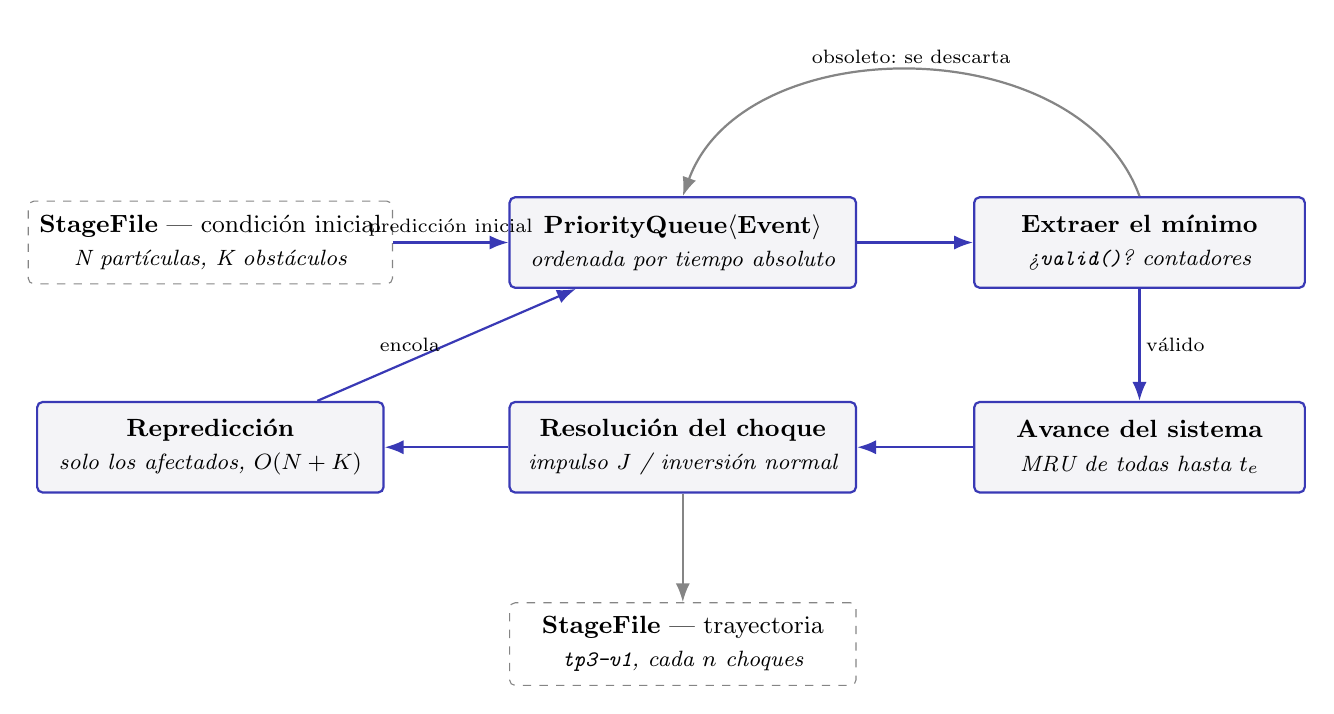
\begin{tikzpicture}[
      node distance=0pt,
      caja/.style={rectangle, rounded corners=2pt, draw=TPBlue, thick,
        fill=TPPlaceholder, align=center, minimum height=1.15cm,
        font=\small, inner sep=4pt},
      externa/.style={rectangle, rounded corners=2pt, draw=TPNavGray, dashed,
        align=center, minimum height=1.05cm, font=\small, inner sep=4pt},
      flecha/.style={-{Latex[length=2.4mm]}, draw=TPBlue, thick},
      flechagris/.style={-{Latex[length=2.4mm]}, draw=TPNavGray, thick},
      etiqueta/.style={font=\scriptsize, inner sep=2pt},
    ]

    \node[externa, minimum width=4.4cm] (ic)     at (0.6,3.1)  {\textbf{StageFile} --- condición inicial\\[1pt]{\footnotesize\itshape N partículas, K obstáculos}};
    \node[caja,    minimum width=4.4cm] (cola)   at (6.6,3.1)  {\textbf{PriorityQueue$\langle$Event$\rangle$}\\[1pt]{\footnotesize\itshape ordenada por tiempo absoluto}};
    \node[caja,    minimum width=4.2cm] (extrae) at (12.4,3.1) {\textbf{Extraer el mínimo}\\[1pt]{\footnotesize\itshape ¿\texttt{valid()}? contadores}};
    \node[caja,    minimum width=4.2cm] (avance) at (12.4,0.5) {\textbf{Avance del sistema}\\[1pt]{\footnotesize\itshape MRU de todas hasta $t_e$}};
    \node[caja,    minimum width=4.4cm] (resol)  at (6.6,0.5)  {\textbf{Resolución del choque}\\[1pt]{\footnotesize\itshape impulso $J$ / inversión normal}};
    \node[caja,    minimum width=4.4cm] (repred) at (0.6,0.5)  {\textbf{Repredicción}\\[1pt]{\footnotesize\itshape solo los afectados, $O(N+K)$}};
    \node[externa, minimum width=4.4cm] (out)    at (6.6,-2.0) {\textbf{StageFile} --- trayectoria\\[1pt]{\footnotesize\itshape \texttt{tp3-v1}, cada $n$ choques}};

    \draw[flecha] (ic)     -- node[etiqueta, above] {predicción inicial} (cola);
    \draw[flecha] (cola)   -- (extrae);
    \draw[flecha] (extrae) -- node[etiqueta, right] {válido} (avance);
    \draw[flecha] (avance) -- (resol);
    \draw[flecha] (resol)  -- (repred);
    \draw[flecha] (repred) -- node[etiqueta, left] {encola} (cola);
    \draw[flechagris] (extrae.north) to[out=110,in=70]
      node[etiqueta, above] {obsoleto: se descarta} (cola.north);
    \draw[flechagris] (resol) -- (out);

  \end{tikzpicture}%
  }
\end{frame}

% ---------------- SIMULACIONES ----------------
% 10
\sectiondivider{Simulaciones}

% 11
% Esquema generado por figuras/plot_geometria_sistema.py (matplotlib) --
% marca L, W, d, r y R_k sobre el dibujo (corrección real de TP2, D9/D11).
% Posiciones de partículas y obstáculos son ilustrativas, no de una
% corrida real. Regenerar con `python3 figuras/plot_geometria_sistema.py`
% si cambia la paleta de colores o el estilo del resto de la deck.
\begin{frame}{Geometría del Sistema}
  \centering
  \maybeimage{figuras/geometria-sistema.png}{5.0cm}{Insertar esquema del sistema con L, W, d, r, $R_k$ marcados}
  \vspace{0.15cm}

  {\small
    \textcolor{TPFresca}{$\bullet$}~Partícula fresca\quad
    \textcolor{TPUsada}{$\bullet$}~Partícula usada\quad
    \textcolor{TPObstaculo}{$\bullet$}~Obstáculo fijo
  \par}
  \vspace{0.08cm}
  {\small\color{TPNavGray} gol si $|y - W/2| \leq d/2$ sobre una pared corta\par}
\end{frame}

% 12
\begin{frame}{Parámetros}
  \small
  Parámetros de entrada fijos:
  \begin{itemize}
    \item $L = 1.20$ m, $W = 0.68$ m
    \item $d = 0.20$ m
    \item $r = 0.0175$ m, $m = 0.025$ kg
    \item $v_0 = 1$ m/s, dirección $\sim U[0,2\pi)$
  \end{itemize}
  Parámetros de entrada variables:
  \begin{itemize}
    \item $N = 100$ (fijado por el enunciado a partir del punto 1.2)
    \item $t_f = 30$ s (tiempo de ejecución)
    \item $K$, $(x_k, y_k, R_k)$: $R_k \geq r$, sin solapamiento
  \end{itemize}
  \vspace{0.1cm}
  \begin{databox}{Nro.\ de realizaciones}
    \centering
    Tiempo de ejecución: 10 \hfill $\langle t_{90}\rangle$: 50 \hfill DCM: 1
  \end{databox}
\end{frame}

% 13
\begin{frame}{Observables}
  \small
  \textbf{Conversión:} $N_g(t)$ = goles acumulados.
  \[
    F_u(t) = \frac{N_g(t)}{N},
    \qquad
    t_{90,r} = \min\{\,t : F_u(t) \geq 0.9\,\}
  \]
  {\scriptsize Si no llega a 0.9 en la realización $r$: se reporta $N_g(t_{\max})$.
  Se reporta el promedio entre $M$ realizaciones,
  $\langle t_{90}\rangle = \frac{1}{M}\sum_{r=1}^{M} t_{90,r}$, con su desvío
  muestral.\par}
  \vspace{0.15cm}

  \textbf{Difusión:} DCM, partículas móviles (frescas+usadas), 1 realización:
  \[
    z(t) = \left\langle \left|\bm{r}_i(t) - \bm{r}_i(0)\right|^2 \right\rangle_i,
    \qquad
    z(t) = c\,t
    \ \Rightarrow\ D = \frac{c}{2}
  \]
  {\scriptsize Pendiente $c$: minimiza
  $E(c) = \sum_k \left(z_k - c\,t_k\right)^2$.\par}
  \vspace{0.15cm}

  \textbf{Costo:} tiempo de ejecución de una realización.
\end{frame}

% ---------------- RESULTADOS ----------------
% 14
\sectiondivider{Resultados}

% 15
\begin{frame}[c]{Tiempo de Ejecución en Función de $N$}
  \resultadofigura{figuras/tiempo-ejecucion-vs-n.png}{4.9cm}{Insertar tiempo de ejecución vs.\ $N$}
    {\item Mesa vacía \item $t_f = 30$ s \item Realizaciones: 10}{}{}
\end{frame}

% 16
\begin{frame}[c]{Mesa Vacía --- Evolución del Sistema}
  \animacionsimple{figuras/vacia_frame.png}{5.1cm}{\animacionVaciaURL}
    {Insertar fotograma representativo de la mesa vacía}
    {\item $N = 100$ \item $K = 0$ \item $t_{\max} = 100$ s}
\end{frame}

% 17
\begin{frame}[c]{Mesa Vacía --- Fracción de Partículas Usadas}
  \resultadofigura{figuras/fu-temporal-vacia.pdf}{4.9cm}{Insertar $F_u(t)$ y la lectura de $t_{90}$}
    {\item $N = 100$ \item $K = 0$ \item 1--2 corridas representativas}{}{}
\end{frame}

% 18
\begin{frame}[c]{Un Obstáculo sobre el Eje Longitudinal}
  \resultadofigura{figuras/t90-vs-xk.png}{4.7cm}{Insertar $\langle t_{90}\rangle$ vs.\ $x_k$}
    {\item $N = 100$ \item $K = 1$, $R = 0.30$ m \item $y_k = W/2$ \item Realizaciones: 50}{}{}
\end{frame}

% 19
\begin{frame}[c]{Un Obstáculo en el Centro --- Radio}
  \resultadofigura{figuras/t90-vs-r-central.png}{4.7cm}{Insertar $\langle t_{90}\rangle$ vs.\ $R$}
    {\item $N = 100$ \item $K = 1$ \item Centro de la mesa \item Realizaciones: 50}
    {figuras/mapa-central.png}{Ej.: $R = 0.34$ m}
\end{frame}

% 20
\begin{frame}[c]{$K$ Obstáculos de Área Total Fija}
  \resultadofigura{figuras/t90-vs-k.pdf}{4.7cm}{Insertar $\langle t_{90}\rangle$ vs.\ $K$}
    {\item $N = 100$ \item $\sum \pi R_k^2$ constante \item Realizaciones: 5}{}{}
\end{frame}

% 21
% Dos bordes para el mismo embudo: discos de radio r sobre la recta
% (frontera lisa) o relleno libre (discos grandes asomando).
\begin{frame}[c]{Embudos hacia los Arcos}
  \resultadofigura{figuras/t90-vs-largo-embudo.png}{4.7cm}{Insertar $\langle t_{90}\rangle$ vs.\ $a$}
    {\item $N = 100$ \item Embudo en ambos arcos \item Realizaciones: 50}
    {figuras/mapa-embudo.png}{Ej.: $a = 0.30$ m}
\end{frame}

% 22
\begin{frame}[c]{Red de Obstáculos Mínimos (Galton)}
  \resultadofigura{figuras/t90-vs-separacion-galton.png}{4.7cm}{Insertar $\langle t_{90}\rangle$ vs.\ $s$}
    {\item $N = 100$ \item $R_k = r$ \item Red triangular \item Realizaciones: 50}
    {figuras/mapa-galton.png}{Ej.: $s = 0.10$ m}
\end{frame}

% 23
% Referencia: disco central R = 0.32 m solo (no la mesa vacía).
\begin{frame}[c]{Disco Central y Cuenco}
  \resultadofigura{figuras/t90-vs-rf-central-cuenco.png}{4.7cm}{Insertar $\langle t_{90}\rangle$ vs.\ $R_f$}
    {\item $N = 100$ \item Disco central\\ $R = 0.32$ m \item Semicírculo libre en cada arco \item Realizaciones: 50}
    {figuras/mapa-central-cuenco.png}{Ej.: $R_f = 0.30$ m}
\end{frame}

% 24
\begin{frame}[c]{Cuenco --- Centro Desplazado}
  \resultadofigura{figuras/t90-vs-desplazamiento-cuenco.png}{4.7cm}{Insertar $\langle t_{90}\rangle$ vs.\ $s$}
    {\item $N = 100$ \item $R_f = 0.35$ m \item Centro a $s$ del arco \item Realizaciones: 50}
    {figuras/mapa-cuenco-desplazado.png}{Ej.: $s = 0.20$ m}
\end{frame}

% 25
% Barrido en curso (cuenco_fino_radio): R_f de 0.28 a 0.58 m, frontera de
% discos de radio r, centro en el arco.
\begin{frame}[c]{Cuenco --- Radio Libre}
  \resultadofigura{figuras/t90-vs-rf-cuenco.png}{4.7cm}{Insertar $\langle t_{90}\rangle$ vs.\ $R_f$}
    {\item $N = 100$ \item Centro en el arco \item Frontera de discos $R_k = r$ \item Realizaciones: 50}{}{}
\end{frame}

% 26
\begin{frame}[c]{Comparación de Arquetipos de Obstáculos}
  \resultadofigura{figuras/t90-vs-arquetipo.pdf}{4.7cm}{Insertar $\langle t_{90}\rangle$ por arquetipo (embudo, cuenco, palos, disco solo) vs.\ mesa vacía}
    {\item $N = 100$ \item Base común: disco central $R = 0.32$ m (salvo cuenco fino) \item Realizaciones: 50}{}{}
\end{frame}

% 27
\begin{frame}[c]{Configuración Elegida --- Evolución del Sistema}
  \animacionsimple{figuras/elegida_frame.png}{5.1cm}{\animacionElegidaURL}
    {Insertar fotograma representativo de la configuración elegida}
    {\item $N = 100$ \item Disco central $R = 0.32$ m \item Cuenco $R_f = 0.30$ m (ambos arcos) \item $t_{\max} = 100$ s}
\end{frame}

% 28
\begin{frame}[c]{Configuración Elegida --- Comparación contra la Mesa Vacía}
  \resultadofigura{figuras/fu-temporal-elegida.pdf}{4.7cm}{Insertar $F_u(t)$ de la configuración elegida y de la mesa vacía}
    {\item $N = 100$ \item Realizaciones: 5}{}{}
\end{frame}

% 29
\begin{frame}[c]{Desplazamiento Cuadrático Medio y Ajuste Lineal}
  \resultadofigura{figuras/dcm-ajuste.pdf}{4.7cm}{Insertar $z(t)$ con el ajuste superpuesto}
    {\item $N = 100$ \item Una realización \item $z = c\,t$, $D = c/2$}{}{}
\end{frame}

% 30
\begin{frame}[c]{Coeficiente de Difusión}
  \resultadofigura{figuras/d-vs-t90.pdf}{4.7cm}{Insertar $D$ vs.\ $\langle t_{90}\rangle$ por configuración}
    {\item $N = 100$ \item Barras de error solo en $\langle t_{90}\rangle$}{}{}
\end{frame}

% ---------------- CONCLUSIONES ----------------
% 31
\sectiondivider{Conclusiones}

% 32
% RECORDATORIOS (correcciones reales de TP2):
%  - Aclarar SIEMPRE a qué configuración se refiere cada afirmación.
%    Nunca "el sistema depende de K" sin decir cómo y en qué configuración.
%  - Si se afirma que D corresponde a un gas, comparar contra un valor
%    tabulado real y citarlo -- no afirmarlo a secas.
%  - No afirmar correlación D--<t90> sin la figura que la sustente.
%  - Nada de hipótesis explicativas que no se hayan estudiado explícitamente.
\begin{frame}{Conclusiones}
  \begin{itemize}
    \item COMPLETAR --- configuración que minimiza $\langle t_{90}\rangle$ y
      cuánto mejora respecto de la mesa vacía.
    \item COMPLETAR --- cómo depende $\langle t_{90}\rangle$ de la variable
      explorada, indicando la configuración.
    \item COMPLETAR --- si existe o no correlación entre $D$ y
      $\langle t_{90}\rangle$, según lo mostrado en la figura.
  \end{itemize}
\end{frame}

% 33. Cierre
\begin{frame}{}
  \vfill
  \begin{beamercolorbox}[wd=0.86\paperwidth,ht=0.72cm,dp=0.20cm,center]{frametitle}
    \LARGE Muchas gracias
  \end{beamercolorbox}
  \vspace{0.4cm}
  \begin{center}
    \maybeimage{figuras/muchas_gracias.jpeg}{3.1cm}{Insertar imagen de cierre}
  \end{center}
  \vfill
\end{frame}

\end{document}
